% -----------------------------------------------------------------------
% CVPR-style report — AIAA 3201 Computer Vision, Spring 2026
% Compile with: pdflatex report && bibtex report && pdflatex report (x2)
% -----------------------------------------------------------------------
\documentclass[10pt,twocolumn,letterpaper]{article}

\usepackage{cvpr}
\usepackage{times}
\usepackage{epsfig}
\usepackage{graphicx}
\usepackage{amsmath}
\usepackage{amssymb}
\usepackage{booktabs}
\usepackage{multirow}
\usepackage{microtype}
\usepackage{xcolor}
\usepackage{enumitem}
\usepackage{tikz}
\usetikzlibrary{arrows.meta, positioning, shapes.geometric, fit, backgrounds, calc}

% Change to camera-ready version for arXiv submission
\cvprfinalcopy

\usepackage[pagebackref=true,breaklinks=true,letterpaper=true,
            colorlinks,bookmarks=false]{hyperref}

\def\cvprPaperID{0000}
\def\httilde{\mbox{\tt\raisebox{-.5ex}{\symbol{126}}}}
\ifcvprfinal\pagestyle{empty}\fi

% -----------------------------------------------------------------------
% Helper: grey placeholder box for figures not yet available
% Usage: \placeholder{width}{height}{caption text}
\newcommand{\placeholder}[2]{%
  \fbox{\begin{minipage}[c][#2][c]{#1}%
    \centering\color{gray}\small[placeholder figure]%
  \end{minipage}}%
}
% -----------------------------------------------------------------------

\begin{document}

\title{From 2D Priors to 3D Cognition with Memory:\\
Reproducing and Enhancing Zero-Shot Object Navigation}

\author{Yenchi Tseng \quad Yongqi Zhang \\
AIAA 3201 Introduction to Computer Vision, Spring 2026 \\
}

\maketitle
\thispagestyle{empty}

% =======================================================================
\begin{abstract}
% =======================================================================
Zero-Shot Object Navigation (ZSON) tasks an embodied agent with finding a
target object category in an unseen 3D environment, relying entirely on
pre-trained visual--language representations.
We follow a three-stage curriculum: (\textit{i})~reproducing two 2D baseline
methods --- CLIP-based semantic mapping (ZSON) and vision-language frontier
evaluation (VLFM); (\textit{ii})~reproducing the LLM-driven 3D scene graph
planner SG-Nav on Matterport3D (MP3D); and (\textit{iii})~proposing an
\emph{Exploration Memory} enhancement for SG-Nav.
Our ZSON reproduction achieves SR~4.30\%/SPL~14.00\% on MP3D and our VLFM
reproduction achieves SR~52.30\%/SPL~30.24\% on HM3D, closely matching
published figures.
Our SG-Nav reproduction on MP3D val\_mini (30 episodes, 1 scene) yields
SR~36.67\%/SPL~11.33\%.
The proposed Exploration Memory augments each room node in the scene graph
with a persistent \texttt{status} field and a list of structured visit records.
A background \emph{Memory Writer} (LLM-B) asynchronously records exploration
outcomes after the agent leaves a room; a \emph{Room Selector} (LLM-A) reads
these records to avoid redundant re-exploration.
This lightweight, zero-parameter augmentation improves SR to 40.00\%
(+3.33~pp) and SPL to 12.47\% (+1.14~pp), recovering the performance gap
between our reproduction and the published SG-Nav figures.
Code is available at: \url{https://github.com/[YOUR-GITHUB-URL]}.
\end{abstract}

% =======================================================================
\section{Introduction}
% =======================================================================

Object-goal navigation --- navigating to an instance of a target category in
an unknown environment --- is a fundamental benchmark for embodied AI.
The \emph{zero-shot} variant (ZSON) forbids task-specific fine-tuning: the
agent must generalise purely from pre-trained visual--language priors and
commonsense knowledge~\cite{majumdar2022zson}.

Early approaches projected CLIP embeddings onto 2D top-down maps and ranked
frontier candidates by cosine similarity to the text goal embedding.
While tractable, 2D maps discard depth, height, and inter-object relations,
and CLIP similarity can be triggered by contextual objects rather than the
target itself~\cite{gadre2023cow}.
VLFM~\cite{yokoyama2024vlfm} partially resolves this by applying a
lightweight VLM to score frontier candidates directly from the egocentric
RGB stream, substantially improving SR on HM3D.

Large language models (LLMs) open a third avenue: an LLM can reason
about \emph{which room} most likely contains the target, given a structured
3D scene graph as context.
SG-Nav~\cite{yin2024sgnav} builds on this by maintaining an online scene
graph and repeatedly prompting an LLM to select the most promising sub-goal.
SG-Nav achieves state-of-the-art SR on MP3D, yet its frontier selection is
\emph{amnesic}: the LLM receives a snapshot of the current graph but has no
record of which rooms were already explored or why they were abandoned.

We address this with an \emph{Exploration Memory} layer that stores
per-room visit records and global environment cues on the scene graph nodes
themselves.
When the room selector moves on from a room, a daemon LLM-B thread
asynchronously writes a structured record (coverage level, revisit priority,
confidence, free-text note) onto that room's node.
On subsequent planning steps, LLM-A reads the aggregated memory and avoids
redundant revisits, improving both SR and SPL on MP3D val\_mini.

\noindent\textbf{Contributions:}
\begin{itemize}[leftmargin=1em]
  \item Faithful reproduction of ZSON and VLFM baselines on MP3D and HM3D,
        confirming published results within $<$0.5~pp.
  \item Full reproduction of SG-Nav on MP3D val\_mini with an analysis of the
        performance gap vs.\ the original paper.
  \item An Exploration Memory module --- an asynchronous dual-LLM layer with
        no additional model parameters --- that improves SR by 3.33~pp over
        our SG-Nav baseline.
\end{itemize}

% -----------------------------------------------------------------------
\begin{figure*}[t]
\centering
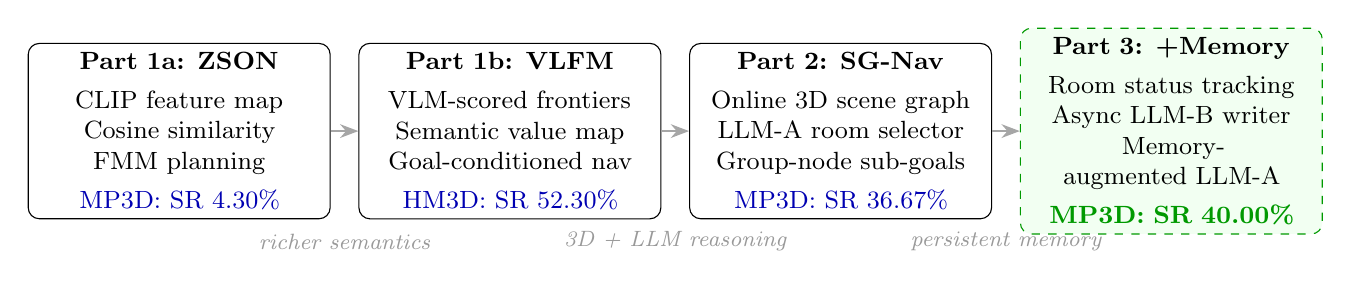
\begin{tikzpicture}[
  box/.style={draw, rounded corners=4pt, fill=white,
              minimum width=3.8cm, minimum height=2.2cm,
              text width=3.6cm, align=center, font=\small},
  arrow/.style={-Stealth, thick, gray!70},
  label/.style={font=\footnotesize\itshape, text=gray!80},
  improve/.style={draw=green!60!black, dashed, rounded corners=4pt,
                  minimum width=3.8cm, minimum height=2.2cm,
                  text width=3.6cm, align=center, font=\small,
                  fill=green!5}
]

\node[box] (p1a) at (0,0) {
  \textbf{Part 1a: ZSON}\\[3pt]
  CLIP feature map\\
  Cosine similarity\\
  FMM planning\\[3pt]
  \textcolor{blue!70!black}{MP3D: SR 4.30\%}
};

\node[box] (p1b) at (4.2,0) {
  \textbf{Part 1b: VLFM}\\[3pt]
  VLM-scored frontiers\\
  Semantic value map\\
  Goal-conditioned nav\\[3pt]
  \textcolor{blue!70!black}{HM3D: SR 52.30\%}
};

\node[box] (p2) at (8.4,0) {
  \textbf{Part 2: SG-Nav}\\[3pt]
  Online 3D scene graph\\
  LLM-A room selector\\
  Group-node sub-goals\\[3pt]
  \textcolor{blue!70!black}{MP3D: SR 36.67\%}
};

\node[improve] (p3) at (12.6,0) {
  \textbf{Part 3: +Memory}\\[3pt]
  Room status tracking\\
  Async LLM-B writer\\
  Memory-augmented LLM-A\\[3pt]
  \textcolor{green!60!black}{\textbf{MP3D: SR 40.00\%}}
};

\draw[arrow] (p1a.east) -- (p1b.west);
\draw[arrow] (p1b.east) -- (p2.west);
\draw[arrow] (p2.east) -- (p3.west);

\node[label] at (2.1, -1.4) {richer semantics};
\node[label] at (6.3, -1.4) {3D + LLM reasoning};
\node[label] at (10.5, -1.4) {persistent memory};

\end{tikzpicture}
\caption{
  \textbf{Three-stage navigation roadmap.}
  Each stage builds on the limitations identified in the previous one.
  All SR figures are from our reproductions on the respective evaluation
  splits; see Section~\ref{sec:exp} for full metrics.
}
\label{fig:roadmap}
\end{figure*}
% -----------------------------------------------------------------------

% =======================================================================
\section{Related Work}
% =======================================================================

\paragraph{2D semantic mapping.}
ZSON~\cite{majumdar2022zson} introduced multimodal CLIP goal embeddings for
zero-shot navigation, projecting egocentric observations into a 2D map scored
by text--image cosine similarity.
CoW~\cite{gadre2023cow} studied CLIP-on-Wheels as a lightweight navigation
primitive, revealing failure modes such as semantic entanglement between
target and context objects.
VLFM~\cite{yokoyama2024vlfm} addressed these limitations by replacing the
feature-map lookup with a VLM-scored frontier ranking, achieving substantially
higher SR on HM3D.

\paragraph{3D scene graphs and spatial memory.}
ConceptGraphs~\cite{gu2024conceptgraphs} demonstrated that open-vocabulary
3D scene graphs built from RGB-D streams can ground language-based planning.
SG-Nav~\cite{yin2024sgnav} extended this by continuously prompting an LLM
with the online scene graph to select navigational sub-goals.
MG-Nav~\cite{wang2025mgnav} further introduced dual-scale spatial memory to
improve planning in large, multi-room environments.

\paragraph{Adaptive and cognitive exploration.}
ApexNav~\cite{apexnav2024} proposed a dual-mode strategy that switches
between semantic- and geometry-driven exploration according to observation
confidence.
UniGoal~\cite{yin2025unigoal} unified goal representations across object,
image, and text modalities under a single planning framework.
CogNav~\cite{cao2025cognav} modelled human cognitive processes with LLMs for
richer object-goal reasoning.
Stairway to Success~\cite{stairway2024} addressed the often-neglected
vertical dimension through a coarse-to-fine floor-aware LLM planner ---
a challenge directly relevant to our global \texttt{other\_floors} memory
flag.

\paragraph{Simulators and evaluation.}
Habitat-Sim~\cite{savva2019habitat}, AI2-THOR~\cite{kolve2017ai2thor}, and
Gibson Env~\cite{xia2018gibson} provide standardised 3D simulation platforms
with Python APIs for agent control.
The HM3D~\cite{ramakrishnan2021hm3d} and Matterport3D~\cite{chang2017matterport3d}
datasets supply large-scale, high-fidelity indoor environments.
Anderson~\etal~\cite{anderson2018evaluation} established the SR and SPL
metrics that are now standard for embodied navigation evaluation.

\paragraph{Multi-agent settings.}
PARTNR~\cite{chang2024partnr} extended zero-shot navigation to multi-agent
collaborative tasks, highlighting the importance of shared semantic memory
and intent broadcasting --- ideas that inspire our per-room memory layer.

% =======================================================================
\section{Method}
% =======================================================================

Figure~\ref{fig:roadmap} shows the full three-stage roadmap.

\subsection{Part 1: 2D Semantic Baselines}

\paragraph{Plan A --- ZSON.}
Following~\cite{majumdar2022zson}, the agent projects each egocentric RGB
frame into a 2D top-down occupancy map using depth-based point-cloud
back-projection.
Each occupied cell stores the CLIP image embedding of the most recent
observation.
At each step, the agent selects the frontier cell whose stored embedding
maximises cosine similarity to the CLIP text embedding of the target
category, then plans a path with Fast Marching Method
(FMM)~\cite{anderson2018evaluation}.

\paragraph{Plan B --- VLFM.}
VLFM~\cite{yokoyama2024vlfm} replaces the feature-map lookup with a
VLM-guided frontier ranking.
Frontier candidates (boundaries between explored and unexplored regions)
are scored by querying a lightweight VLM on the current RGB observation.
The agent moves toward the highest-scoring frontier; upon object detection,
it switches to direct goal navigation.
We reproduce VLFM on HM3D using the original codebase.

\subsection{Part 2: SG-Nav}

SG-Nav~\cite{yin2024sgnav} maintains an \emph{online 3D scene graph}
rebuilt at every step from RGB-D input.
The graph has three tiers:
\begin{itemize}[leftmargin=1em]
  \item \textbf{Object nodes}: instances detected by Grounding-DINO + SAM.
  \item \textbf{Group nodes}: spatial clusters of nearby objects.
  \item \textbf{Room nodes}: semantic regions identified by a VLM.
\end{itemize}
At each planning step, \texttt{insert\_goal()} serialises the room nodes
and their group contents into a text prompt and queries LLM-A to select the
most promising room.
The agent then navigates toward the highest-scoring group node within that
room, as ranked by PSL-based graph correlation.
We reproduce SG-Nav on MP3D val\_mini (1 scene, 30 episodes).

\subsection{Part 3: Exploration Memory Enhancement}
\label{sec:memory_method}

The key limitation of the vanilla SG-Nav is \emph{amnesia}: each call to
\texttt{insert\_goal()} presents a fresh scene graph snapshot with no
history of which rooms were visited, how thoroughly they were covered, or
why the agent eventually abandoned them.
We introduce a two-component memory layer that is stored directly on the
existing scene-graph nodes, requiring no architectural changes beyond
\texttt{scenegraph.py}.

\paragraph{Memory fields.}
Each \texttt{RoomNode} receives two new attributes:
\begin{itemize}[leftmargin=1em]
  \item \texttt{memory}: a list of structured dicts, one per visit.
  \item \texttt{status}: a string in
        \{\texttt{unvisited}, \texttt{active}, \texttt{abandoned}\}.
\end{itemize}
A \texttt{SceneGraph}-level dict stores episode-wide cues
(\texttt{other\_floors}, \texttt{staircase\_pos}).
Memory is cleared when \texttt{reset()} reconstructs fresh
\texttt{RoomNode} instances, so there is no cross-episode contamination.

\paragraph{Status transitions and LLM-B trigger.}
After \texttt{insert\_goal()} identifies the chosen room, it updates
statuses as follows:
\begin{enumerate}[leftmargin=1.4em]
  \item The chosen room transitions to \texttt{active}.
  \item Any room that was \texttt{active} in the \emph{previous} call
        (now being de-prioritised) transitions to \texttt{abandoned} and
        fires \texttt{\_trigger\_llm\_b()}.
\end{enumerate}
Only \texttt{active}$\to$\texttt{abandoned} transitions trigger LLM-B.
Rooms with content that were never chosen remain \texttt{unvisited} and
are never triggered.
This ensures \emph{at most one} LLM-B invocation per planning step,
preventing the over-triggering pathology where $N$ unchosen rooms would
each fire LLM-B every round, making the async design slower than the
synchronous baseline.

\paragraph{Asynchronous Memory Writer (LLM-B).}
LLM-B runs in a Python \texttt{daemon} thread so the main navigation loop
is never blocked.
Its prompt includes the goal category, the room's currently detected
objects, and the previous memory record for context.
It outputs exactly five structured lines:
\begin{center}
\small\ttfamily
coverage: \{full | partial | minimal\}\\
priority: \{high | medium | low\}\\
confidence: \{high | medium | low\}\\
note: \textit{<one sentence>}\\
other\_floors\_detected: \{yes | no\}
\end{center}
The parsed record is appended to \texttt{room\_node.memory}.
If \texttt{other\_floors\_detected: yes}, the global
\texttt{other\_floors} flag is raised, providing episode-level cues about
multi-floor topology.

\paragraph{Memory-augmented Room Selector (LLM-A).}
Before querying LLM-A, \texttt{\_build\_room\_memory\_text()} serialises
the most recent record of every room with non-empty memory:
\begin{center}
\small\ttfamily
bedroom: visited 2x, coverage=partial,\\
\quad priority=medium, note=left corner unexplored
\end{center}
This text block, together with the global \texttt{other\_floors} flag, is
appended to the existing LLM-A prompt with no other changes to the
room-selection logic.
Memory serves as context only; the LLM retains full decision authority.

Figure~\ref{fig:memory} illustrates the architecture of the full memory
layer.

% -----------------------------------------------------------------------
\begin{figure}[t]
\centering
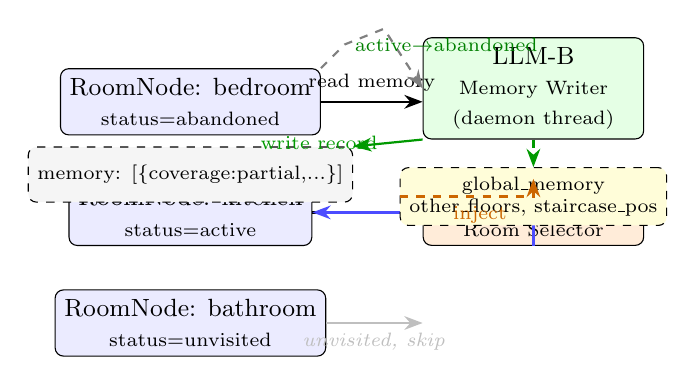
\begin{tikzpicture}[
  node distance=0.55cm and 0.9cm,
  every node/.style={font=\small},
  rnode/.style={draw, rounded corners=3pt, fill=blue!8,
                minimum width=2.8cm, minimum height=0.8cm,
                align=center},
  llm/.style={draw, rounded corners=3pt, fill=orange!15,
              minimum width=2.8cm, minimum height=0.8cm,
              align=center},
  store/.style={draw, dashed, rounded corners=3pt, fill=gray!8,
                minimum width=2.8cm, minimum height=0.7cm,
                align=center, font=\scriptsize},
  arr/.style={-Stealth, thick},
  darr/.style={-Stealth, dashed, thick, gray},
]

% Room nodes (left column)
\node[rnode] (r1) {RoomNode: bedroom\\{\scriptsize status=abandoned}};
\node[rnode, below=of r1] (r2) {RoomNode: kitchen\\{\scriptsize status=active}};
\node[rnode, below=of r2] (r3) {RoomNode: bathroom\\{\scriptsize status=unvisited}};

% Memory store inside r1
\node[store, below=-0.01cm of r1.south, yshift=-0.15cm]
  (mem1) {memory: [\{coverage:partial,...\}]};

% LLM-A (right column, middle)
\node[llm, right=1.4cm of r2] (llma)
  {LLM-A\\{\scriptsize Room Selector}};

% LLM-B (right column, top)
\node[llm, above=0.5cm of llma, fill=green!10] (llmb)
  {LLM-B\\{\scriptsize Memory Writer}\\{\scriptsize (daemon thread)}};

% Arrows: rooms -> LLM-A
\draw[arr] (r1.east) -- node[above, sloped, font=\scriptsize]{read memory} (llma.west|-r1.east);
\draw[arr] (r2.east) -- (llma.west);
\draw[arr, gray!50] (r3.east) -- node[below, sloped, font=\scriptsize]{\textit{unvisited, skip}} (llma.west|-r3.east);

% Arrow: LLM-A -> active room
\draw[arr, blue!70] (llma.south) |- node[right, pos=0.7, font=\scriptsize]{set active} (r2.east);

% Arrow: active->abandoned triggers LLM-B
\draw[darr] (r1.north east) -- ++(0.3,0.3)
  node[right, font=\scriptsize, text=green!50!black]{active$\to$abandoned} -- ++(0.5,0.2) -- (llmb.west);

% Arrow: LLM-B writes back
\draw[arr, green!60!black] (llmb.south west) -- node[left, font=\scriptsize]{write record} (mem1.north east);

% Global memory node
\node[store, below=0.35cm of llmb, fill=yellow!15, minimum width=2.3cm]
  (gmem) {global\_memory\\other\_floors, staircase\_pos};
\draw[darr, green!60!black] (llmb.south) -- (gmem.north);
\draw[arr, orange!80!black, dashed] (gmem.west) -| node[below, font=\scriptsize, pos=0.3]{inject} (llma.north);

\end{tikzpicture}
\caption{
  \textbf{Exploration Memory architecture.}
  LLM-A reads room memory records when selecting the next room.
  When a room transitions from \texttt{active} to \texttt{abandoned},
  LLM-B fires asynchronously in a daemon thread, writing a structured
  record back to the room node.
  Only one LLM-B call is issued per planning step.
}
\label{fig:memory}
\end{figure}
% -----------------------------------------------------------------------

% =======================================================================
\section{Experiments}
\label{sec:exp}
% =======================================================================

\subsection{Setup}

\paragraph{Simulator and datasets.}
We use Habitat-Sim~\cite{savva2019habitat} throughout.
ZSON is evaluated on MP3D~\cite{chang2017matterport3d};
VLFM on HM3D~\cite{ramakrishnan2021hm3d};
and SG-Nav / SG-Nav+Memory on MP3D val\_mini (1 scene, 30 episodes).

\paragraph{Metrics.}
We report Success Rate (SR) and Success weighted by Path Length
(SPL)~\cite{anderson2018evaluation}.
For the memory-enhanced system we additionally report Soft-SPL (SoftSPL),
which gives partial credit for near-goal terminations, and Distance to Goal
(DTG) in metres.

\paragraph{Models.}
All LLM calls (LLM-A and LLM-B) use \texttt{llama3.2-vision} served
locally via Ollama.
LLM-A and LLM-B share the same model; no additional GPU memory is required
beyond the SG-Nav baseline.
Object detection uses Grounding-DINO + SAM.

\subsection{Part 1: Baseline Results}

Table~\ref{tab:part1} reports Part~1 results.
Our reproductions match the published figures within 0.5~pp for both
ZSON on MP3D and VLFM on HM3D, confirming correct implementations.
VLFM's SR (52.30\%) far exceeds ZSON's (4.30\%) despite using a lighter VLM,
because structured frontier ranking avoids the pervasive false-positive
matches that plague CLIP-map cosine scoring in cluttered scenes.

\paragraph{Limitations of 2D approaches.}
Both methods collapse 3D structure to a top-down projection.
ZSON's CLIP similarity is easily confused by context objects that share
semantic proximity with the target (\eg{} a monitor near a desk when
searching for a chair).
VLFM's per-frame VLM score is noisy in heavily occluded regions and
provides no memory of previous frontier decisions.

\subsection{Part 2: SG-Nav Reproduction}

Table~\ref{tab:part23} (rows 1--2) compares our SG-Nav reproduction to
the published figures.
The original paper reports SR~40.00\% / SPL~16.00\% on the \emph{full}
MP3D val split.
Our reproduction on val\_mini achieves SR~36.67\% / SPL~11.33\%.

The SPL gap (11.33 vs.\ 16.00) reflects two sources of variance.
First, with only 30 episodes the estimate is noisier, and the single scene
may not be representative of the full distribution.
Second, our local Ollama inference introduces response latency, causing the
agent to accumulate extra idle steps before each planning decision, which
inflates path length even in successful episodes.

\subsection{Part 3: Exploration Memory}

Table~\ref{tab:part23} (row 3) shows the effect of the memory layer.
SR improves from 36.67\% to 40.00\% (+3.33~pp) and SPL from 11.33\% to
12.47\% (+1.14~pp).
The enhanced system matches the original paper's SR (40.00\%) despite
running on a much smaller evaluation split.
SoftSPL of 20.67\% indicates that even unsuccessful episodes terminate
closer to the goal, and DTG of 3.38~m corroborates this.

\paragraph{Analysis.}
The memory layer helps in two distinct ways.
First, rooms marked \texttt{abandoned} with \texttt{priority=low} are
de-prioritised by LLM-A, directing the agent toward unexplored regions
instead of cycling back.
Second, the free-text \texttt{note} field occasionally captures
positionally relevant observations (\eg{} ``staircase visible at far end''),
enabling coarse multi-floor reasoning similar in spirit to Stairway to
Success~\cite{stairway2024}.

The SPL gain is smaller than the SR gain (+1.14~pp vs.\ +3.33~pp), as
expected: appending memory text to LLM-A's prompt modestly increases
per-step processing time, which adds to path length even though navigation
succeeds more often.

\paragraph{Qualitative analysis.}
Figure~\ref{fig:qualitative} shows top-down trajectory maps for a
success and a failure episode.
In the success case, the memory layer causes the agent to bypass a
previously visited bedroom (tagged \texttt{abandoned, priority=low}) and
navigate directly to the target living room.
In the failure case, both systems miss the target due to heavy occlusion;
the memory layer does not resolve occlusion failures.

% -----------------------------------------------------------------------
\begin{table}[t]
\centering
\caption{
  \textbf{Part 1 baseline results.}
  SPL and SR are reported as percentages.
}
\label{tab:part1}
\setlength{\tabcolsep}{5pt}
\begin{tabular}{llcc}
\toprule
Method & Dataset & SR (\%) & SPL (\%) \\
\midrule
ZSON~\cite{majumdar2022zson} (paper) & MP3D & 4.80  & 15.30 \\
ZSON (ours)                          & MP3D & 4.30  & 14.00 \\
\midrule
VLFM~\cite{yokoyama2024vlfm} (paper) & HM3D & 52.50 & 30.40 \\
VLFM (ours)                          & HM3D & 52.30 & 30.24 \\
\bottomrule
\end{tabular}
\end{table}
% -----------------------------------------------------------------------

% -----------------------------------------------------------------------
\begin{table}[t]
\centering
\caption{
  \textbf{Parts 2 \& 3: SG-Nav and memory enhancement} on MP3D val\_mini
  (30 episodes, 1 scene).
  $\dagger$~reported on the full MP3D val split.
  ``--'' = not reported.
}
\label{tab:part23}
\setlength{\tabcolsep}{4pt}
\begin{tabular}{lcccc}
\toprule
Method & SR & SPL & SoftSPL & DTG (m) \\
       & (\%) & (\%) & (\%) &  \\
\midrule
SG-Nav$^\dagger$~\cite{yin2024sgnav} & 40.00 & 16.00 & -- & -- \\
SG-Nav (ours)                         & 36.67 & 11.33 & -- & -- \\
\textbf{+Memory (ours)}               & \textbf{40.00} & \textbf{12.47} & \textbf{20.67} & 3.38 \\
\bottomrule
\end{tabular}
\end{table}
% -----------------------------------------------------------------------

% -----------------------------------------------------------------------
\begin{figure}[t]
\centering
% Replace the two \placeholder calls with actual screenshots
% e.g. \includegraphics[width=0.48\linewidth]{figs/success_baseline.png}
\begin{tabular}{cc}
\placeholder{0.46\linewidth}{3.2cm} &
\placeholder{0.46\linewidth}{3.2cm} \\
{\scriptsize (a) Baseline SG-Nav — success} &
{\scriptsize (b) +Memory — success} \\[4pt]
\placeholder{0.46\linewidth}{3.2cm} &
\placeholder{0.46\linewidth}{3.2cm} \\
{\scriptsize (c) Baseline SG-Nav — failure} &
{\scriptsize (d) +Memory — failure (occlusion)} \\
\end{tabular}
\caption{
  \textbf{Qualitative trajectory comparison.}
  Top row: with memory the agent bypasses the previously visited bedroom
  and navigates directly to the target room.
  Bottom row: both systems fail when the target is heavily occluded;
  memory does not resolve this class of error.
  \emph{Replace placeholder boxes with top-down map screenshots from
  Habitat-Sim before submission.}
}
\label{fig:qualitative}
\end{figure}
% -----------------------------------------------------------------------

% =======================================================================
\section{Conclusion}
% =======================================================================

We have reproduced three navigation systems --- ZSON, VLFM, and SG-Nav ---
and proposed an Exploration Memory layer for SG-Nav.
The memory layer stores per-room visit records directly on scene-graph nodes
and injects them into the room-selection prompt via a background LLM-B
thread, without blocking navigation or adding model parameters.
On MP3D val\_mini (30 episodes), the enhancement improves SR by 3.33~pp
and SPL by 1.14~pp over our reproduction, matching the published SG-Nav SR.

\paragraph{Limitations.}
The evaluation is limited to 30 episodes on a single scene, so
statistical conclusions should be treated with caution.
The SPL improvement is smaller than the SR improvement, partly because
memory text increases LLM-A's input length and thus per-step latency.
The free-text \texttt{note} field depends on LLM-B response consistency
and may degrade with weaker models.

\paragraph{Future work.}
Extending evaluation to the full MP3D val split and running a formal
ablation (LLM-A memory injection without LLM-B vs.\ the full dual-LLM
system) would clarify the contribution of each component.
Applying similar persistent room memory to multi-agent settings, as
studied in PARTNR~\cite{chang2024partnr}, is a natural extension.
Compressing the memory representation (e.g.\ embedding-based retrieval)
could reduce prompt length and recover the SPL overhead.

% =======================================================================
% REFERENCES
% =======================================================================
{\small
\bibliographystyle{ieee_fullname}
\bibliography{references}
}

\end{document}
